\section{Introduction} %\label{sec:extenstion_introduction}

This chapter extends the previous work in \cite{calderon_scalable_2023}. The main new contributions are summarized as follows. First, we introduce a new spatial partitioner, based on the kd-tree partitioning strategy, for constructing overlay  DCELs (section \ref{sec:pstrategies}). Since it better utilizes the data distributions in optimizing DCEL partitions, it leads to noticeably improved performance. The new partitioning strategy contrasts with the original strategy that employed space-partitioning techniques based on quadtrees. 

Second, we extend the overlay DCEL approach to accept scattered and noisy line segments as input, rather than being restricted to clean polygon data. This enhancement builds on the scalable polygonization methods presented in \cite{abdelhafeez_ddcel_2023}, enabling the overlay of real-world datasets composed of vast sets of line segments —datasets that existing techniques are unable to process effectively.

For instance, Figure \ref{fig:extension_dcel_example} illustrates the fundamental components of a DCEL. Additionally, we identify two types of special half-edges. \textit{Dangles} are half-edges with one or both endpoints not incident on another half-edge endpoint; both half-edge $\overrightarrow{fj}$ and its twin are considered dangle edges. \textit{Cut-edges} are half-edges connected at both ends that do not form part of any polygon. The half-edge $\overrightarrow{dg}$ and its twin are classified as cut-edges.

\begin{figure}
    \centering
    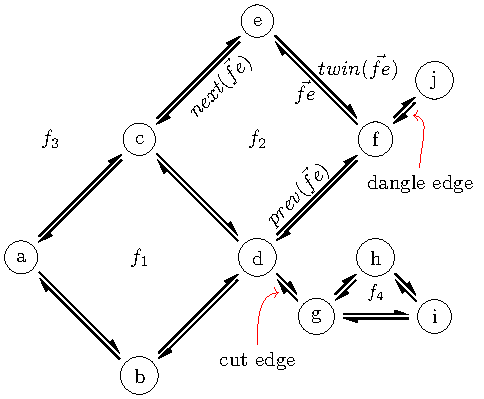
\includegraphics[width=0.6\linewidth]{chapterExtension/dcel_example2}
    \caption{Components of the DCEL structure with dangle and cut edges.}\label{fig:extension_dcel_example}
\end{figure}

The remainder of this chapter is organized as follows. Section \ref{sec:extension_methods} details the implementation of the new kd-tree partitioner and describes the polygon extraction process for adapting line segment inputs, which extends the overlay method to support dangle and cut edges. In Section \ref{sec:extension_experiments}, we present additional experiments to quantify the benefits of the kd-tree-based strategy and assess the performance of the proposed polygonization on datasets with large volumes of line segments.
